\section{Symulacja CFD}
\subsection{Opis problemu}
Drony podwodne typu glider typowo poruszają się w trajektorii piło-kształtnej lub trójkątnej, przy czym w punktach ekstremalnych ruchu trajektoria może przyjmować charakter sinusoidalny (przejście z 

W związku z tym symulację CFD wydzielono na 3 


\subsection{Domena}
Na podstawie wcześniej przygotowanej geometrii drona opartej o model DARPA Suboff Hull, ze skrzydłami o profilu Clark-Y i statecznikami o profilu NACA J5012 przygotowano domenę.\cite{dron-main}. 

Z uwagi na konieczność zbadania sił przy różnych wartościach kątą natarcia $\alpha$ drona oraz zbadania sił występujących przy ruchu przechylającym domena została podzielona na objętość zewnętrzną i objętość wewnętrzną z geometrią badanego drona. Objętość wewnętrzną stanowił walec położony na środku układu współrzędnych, o średnicy D = 2 m i wysokości H = 1 m, natomiast objętość zewnętrzną stanowił prostopadłościan, w którym wlot znajdował się w odległości 5 długości L, wylot 10 długości L, ścianki domeny 5 długości L od środka układu współrzędnych, domenę i jej wymiary przedstawiono na rys. \ref{fig:domain}.

Zastosowanie siatki typu non-conformal mesh pozwoliło na przygotowanie siatki strukturalnej dla objętości zewnętrznej i proste sterowanie kątem natarcia $\alpha$ oraz w dalszej części sterowanie prędkością kątową drona $\omega$.

\ref{fig:domain}.            
\begin{figure}[H]
	\centering
	
\includegraphics[width=0.8\linewidth]{pictures/dummy.png}
	\caption{Domena - widok ogólny}
	\label{fig:domain}
\end{figure}


\subsection{Siatka}
\subsubsection{Test zbieżności siatki}
W celu sprawdzenia czy wyniki symulacji są niezależne od wielkości siatki przeprowadzono test zbieżności siatki. Test przeprowadzono poprzez kolejno zmniejszanie elementów siatki aż różnice między wynikami były pomijalnie małe (przyjęto $\Delta<1\%$). Wyniki testu zbieżności zawarto w tabeli \ref{tab:convergence} oraz przedstawiono na wykresie \ref{fig:convergence}.

\begin{table}[H]
	\centering
	\caption{Zbieżność siatki}
	\label{tab:convergence}
	\begin{tabular}{*{9}{l}} % You can use this syntax to create multiple columns just by changing the number.
		\toprule
		Siatka & size [mm] & count & cl & cd & cm & $\delta\text{cl}$ & $\delta\text{cd}$ & $\delta\text{cm}$\\ \midrule
		Zgrubna & 1600 & 6,93E+05 & 0.249 & 0.032 & -0.0153 & - & - & - \\ \midrule
		Średnia & 800 & 7,86E+05 & 0.223 & 0.031 & -0.0149 & 10.44\% & 3.13\% & 2.61\% \\ \midrule
		Dokładna & 400 & 9,32E+05 & 0.224 & 0.030 & -0.0148 & 0.44\% & 0.32\% & 0.67\% \\ \midrule
		Bardzo dokładna & 200 & 1,65E+06 & 0.223 & 0.029 & -0.0146 & 0.44\% & 0.33\% & 1.35\% \\ \midrule    Bardzo dokładna & 100 & 1,65E+06 & 0.223 & 0.029 & -0.0146 & 0\% & 0\% & 0\% \\ 
		
		\bottomrule
	\end{tabular}
\end{table}

\begin{figure}[H]
	\centering
	\begin{subfigure}[b]{0.45\textwidth}
		\centering
		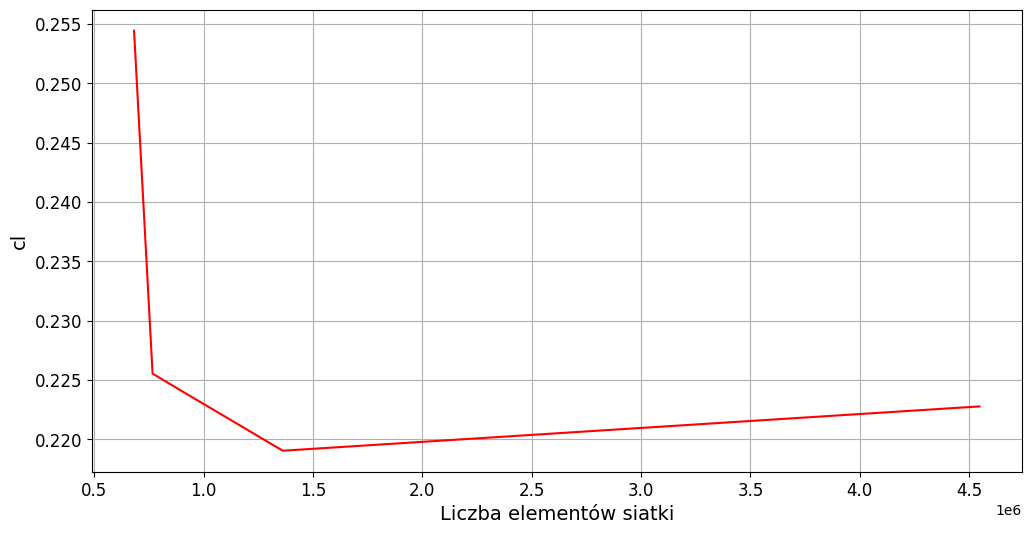
\includegraphics[width=1\linewidth]{pictures/cl-conv.png}
		\caption{Wykres zbieżności cl.}
	\end{subfigure}
	\begin{subfigure}[b]{0.45\textwidth}
		\centering
		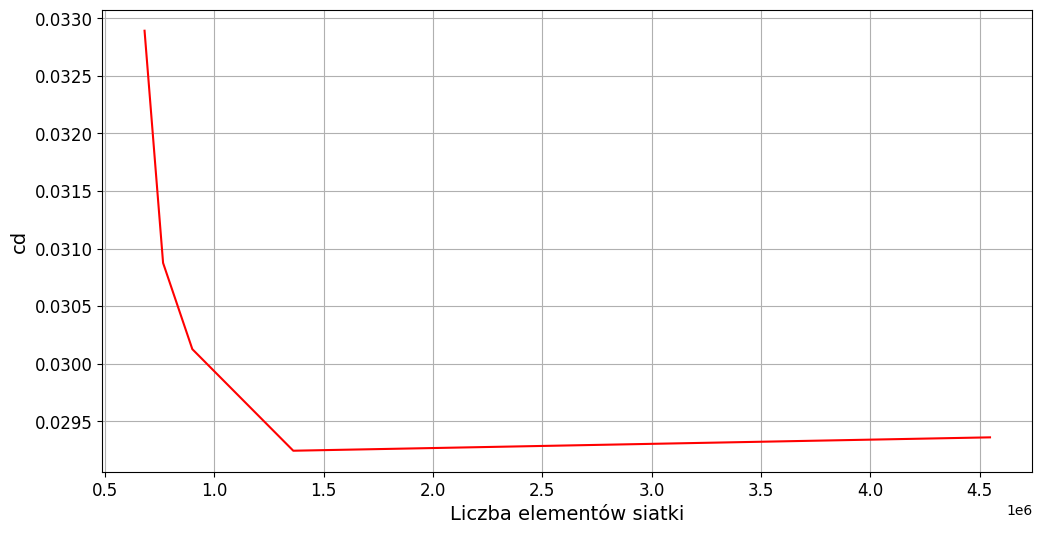
\includegraphics[width=1\linewidth]{pictures/cd-conv.png}
		\caption{Wykres zbieżności cd.}
	\end{subfigure}
	\begin{subfigure}[b]{0.45\textwidth}
		\centering
		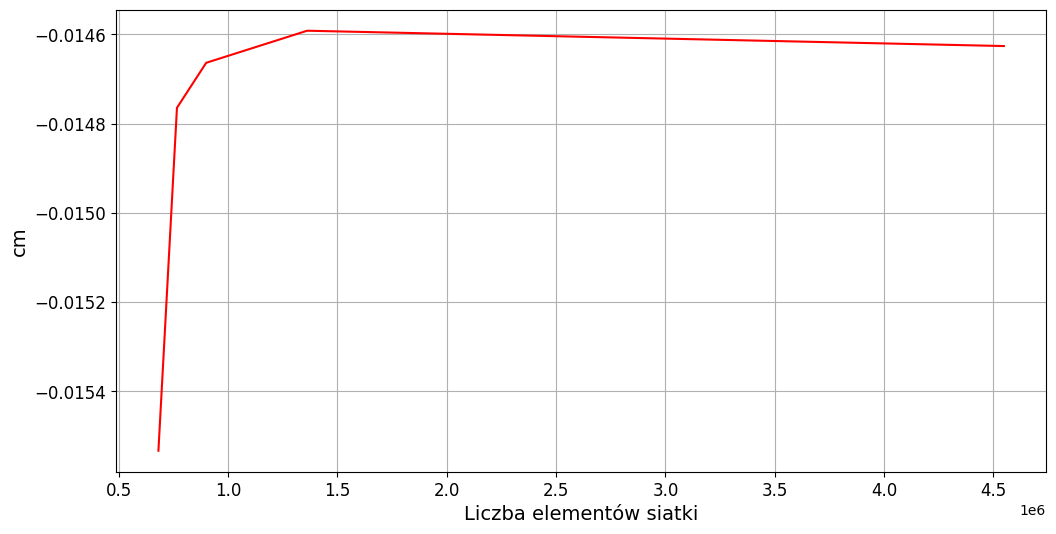
\includegraphics[width=1\linewidth]{pictures/cm-conv.png}
		\caption{Wykres zbieżności cm.}
	\end{subfigure}
	\caption{Wykresy zbieżności.}
	\label{fig:convergence}
\end{figure}

Z uwagi na małe zmiany między wynikami siatek medium, medium-fine i fine, uznano siatkę medium-fine za wystarczająco dokładną i w celu ograniczenia czasu trwania obliczeń została ona zastosowana do dalszych symulacji.
\subsubsection{Ustawienia symulacji}

\subsubsection{y+}
W celu zamodelowania warstwy przyściennej za pomocą funkcji przyściennych (wall functions), dodano 10 warstw inflacyjnych w okół geometrii drona.

Dobrano wysokości pierwszej warstwy inflacyjnej tak aby uzyskać wartości $\text{y+}\in(30; 300)$ dla zakresu prędkości $v\in(0.5\text{m/s}; 1,5\text{m/s}$, wysokości pierwszej warstwy dla danych prędkości zestawiono w tabeli \ref{tab:first-layer-heights}, natomiast histogramy y+ przedstawiono na rys. \ref{fig:histograms}.   Na rysunku \ref{fig:yplus-contours} przedstawiono wartości y+ na powierzchniach kadłuba, skrzydeł i stateczników drona.

\begin{table}[H]
	\centering
	\caption{Mesh convergence}
	\label{tab:first-layer-heights}
	\begin{tabular}{*{2}{l}} % You can use this syntax to create multiple columns just by changing the number.
		\toprule
		v [m/s] & $\text{y}_0$ [mm] \\ \midrule
		0,5 & 3,0 \\ \midrule
		0,7 & 2,5 \\ \midrule
		1,5 & 2,5 \\ 
		\bottomrule
	\end{tabular}
\end{table}

\begin{figure}[H]
	\centering
	\begin{subfigure}[b]{0.4\textwidth}
		\centering
		
\includegraphics[width=1\linewidth]{pictures/dummy.png}
		\caption{Histogram y+ dla $\text{v}=0.5 \ \text{m/s}$}
	\end{subfigure}
	\begin{subfigure}[b]{0.4\textwidth}
		\centering
		
\includegraphics[width=1\linewidth]{pictures/dummy.png}
		\caption{Histogram y+ dla $\text{v}=0.7 \ \text{m/s}$}
	\end{subfigure}
	\begin{subfigure}[b]{0.4\textwidth}
		\centering
		
\includegraphics[width=1\linewidth]{pictures/dummy.png}
		\caption{Histogram y+ dla $\text{v}=1.5 \ \text{m/s}$}
	\end{subfigure}
	\caption{Histogram wartości y+}
	\label{fig:histograms}
\end{figure}

\begin{figure}[H]
	\centering
	\begin{subfigure}[b]{0.4\textwidth}
		\centering
		
\includegraphics[width=1\linewidth]{pictures/dummy.png}
		\caption{Wartości y+ dla $\text{v}=0.5 \ \text{m/s}$}
	\end{subfigure}
	\begin{subfigure}[b]{0.4\textwidth}
		\centering
		
\includegraphics[width=1\linewidth]{pictures/dummy.png}
		\caption{Wartości y+ dla $\text{v}=0.7 \ \text{m/s}$}
	\end{subfigure}
	\begin{subfigure}[b]{0.4\textwidth}
		\centering
		
\includegraphics[width=1\linewidth]{pictures/dummy.png}
		\caption{Wartości y+ dla $\text{v}=1.5 \ \text{m/s}$}
	\end{subfigure}
	\caption{Wartości y+ na powierzchniach drona}
	\label{fig:yplus-contours}
\end{figure}


\subsubsection{Walidacja z poprzednio przeprowadzonymi symulacjami}
W celu potwierdzenia powtarzalności z poprzednio przeprowadzonymi symulacjami przeprowadzono wstępne badanie współczynników cl, cd, cm względem kąta natarcia $\alpha$.
Badanie przeprowadzono dla zakresu kąta natarcia $\alpha\in(0^\circ; 15^\circ)$ ze skokiem $\Delta\alpha=2,5^\circ$, przy prędkości przepływu $\text{v}=\text{0.7 m/s}$. Wyniki porównano z wynikami poprzednio przeprowadzonych symulacji\cite{dron-main} i zestawiono w tabeli \ref{tab:validation}, ich charakterystyki wraz z wykresami błędów względnych przedstawiono na rys \ref{fig:validations}.

\begin{table}[H]
	\centering
	\caption{Mesh convergence}
	\label{tab:validation}
	\begin{tabular}{*{10}{l}} % You can use this syntax to create multiple columns just by changing the number.
		\toprule
		$\alpha $& cl & cd & cm & cl\_prev & cd\_prev & cm\_prev & $\delta\text{cl}$ & $\delta\text{cd}$ & $\delta\text{cm}$ \\ \midrule 
		0 & 0,224 & 0,030 & -0,0147 & 0,226 & 0,028 & -0,015 & 0,89\% & 7,14\% & 0\% \\ \midrule
		2,5 & 0,314 & 0,038, & -0,0261 & 0,322 & 0,035 & -0,027 & 2,48\% & 8,57\% & 8,67\% \\ \midrule
		5 & 0,372 & 0,051 & -0,0337 & 0,402 & 0,047 & -0,036 & 14,70\% & 7,84\% & 6,39\% \\ \midrule
		7,5 & 0,402 & 0,071 & -0,0368 & 0,422 & 0,067 & -0,036 & 4,74\% & 5,97\% & 2,22\% \\ \midrule
		10 & 0,417 & 0,094 & -0,0340 & 0,443 & 0,092 & -0,039 & 5,87\% & 2,17\% & 12,82\% \\ \midrule
		12,5 & 0,435 & 0,122 & -0,040 & 0,458 & 0,119 & -0,041 & 5,02\% & 2,52\% & 2,44\% \\ \midrule
		15 & 0,454 & 0,150 & -0,0428 & 0,471 & 0,146 & -0,044 & 3,61\% & 2,74\% & 2,73\% \\ 
		
		\bottomrule
	\end{tabular}
\end{table}

\begin{figure}[H]
	\centering
	\begin{subfigure}[b]{0.4\textwidth}
		\centering
		
\includegraphics[width=1\linewidth]{pictures/dummy.png}
		\caption{Wykres charakterystyki cl.}
	\end{subfigure}
	\begin{subfigure}[b]{0.4\textwidth}
		\centering
		
\includegraphics[width=1\linewidth]{pictures/dummy.png}
		\caption{Wykres błędów względnych cl.}
	\end{subfigure}
	\begin{subfigure}[b]{0.4\textwidth}
		\centering
		
\includegraphics[width=1\linewidth]{pictures/dummy.png}
		\caption{Wykres charakterystyki cd.}
	\end{subfigure}
	\begin{subfigure}[b]{0.4\textwidth}
		\centering
		
\includegraphics[width=1\linewidth]{pictures/dummy.png}
		\caption{Wykres błędów względnych cd.}
	\end{subfigure}
	\begin{subfigure}[b]{0.4\textwidth}
		\centering
		
\includegraphics[width=1\linewidth]{pictures/dummy.png}
		\caption{Wykres charakterystyki m.}
	\end{subfigure}
	\begin{subfigure}[b]{0.4\textwidth}
		\centering
		
\includegraphics[width=1\linewidth]{pictures/dummy.png}
		\caption{Wykres błędów względnych cm.}
	\end{subfigure}
	
	
	\caption{Wykresy uzyskanych charakterystyk cl, cd, cm oraz błędów względnych dla zakresów kąta natarcia $\alpha\in(0^\circ, 15^\circ)$.}
	\label{fig:validations}
\end{figure}

Błędy względne między przygotowaną symulacją a poprzednio przeprowadzonymi symulacjami były stosunkowo małe (w okolicach $\max{\delta}=10\%$, przygotowany model uznano więc za wystarczająco dokładny do dalszych obliczeń.

\subsection{Wybranie zakresów operacyjnych kąta natarcia drona}
W celu określenia zakresów kąta natarcia w jakich dron będzie pracował przeprowadzon obadanie sprawności hydrodynamicznej drona, czyli stosunku cl/cd współczynników siły nośnej cl i oporu cd. W tym celu przeprowadzono symulację dla zakresu kąta natarcia $\alpha=[-35^\circ, 35^\circ]$ ze skokiem o $\Delta\alpha=2,5^\circ$, przy prędkości przepływu $\text{v}=0.7 \ \text{m/s}$. Uzyskane wykresy charakterystyk współczynników siły nośnej cl, oporu cd i stosunku cl/cd przedstawiono na rysunku \ref{fig:efficiency-graphs}, natomiast kontury prędkości, ciśnienia statycznego i dynamicznego dla wybranych wartości kąta $\alpha=0^\circ, \pm10^\circ, \pm20^\circ, \pm30^\circ$ przedstawiono na rysunku \ref{fig:efficiency-pics}. 

\begin{figure}[H]
	\centering
	\begin{subfigure}[b]{0.4\textwidth}
		\centering
		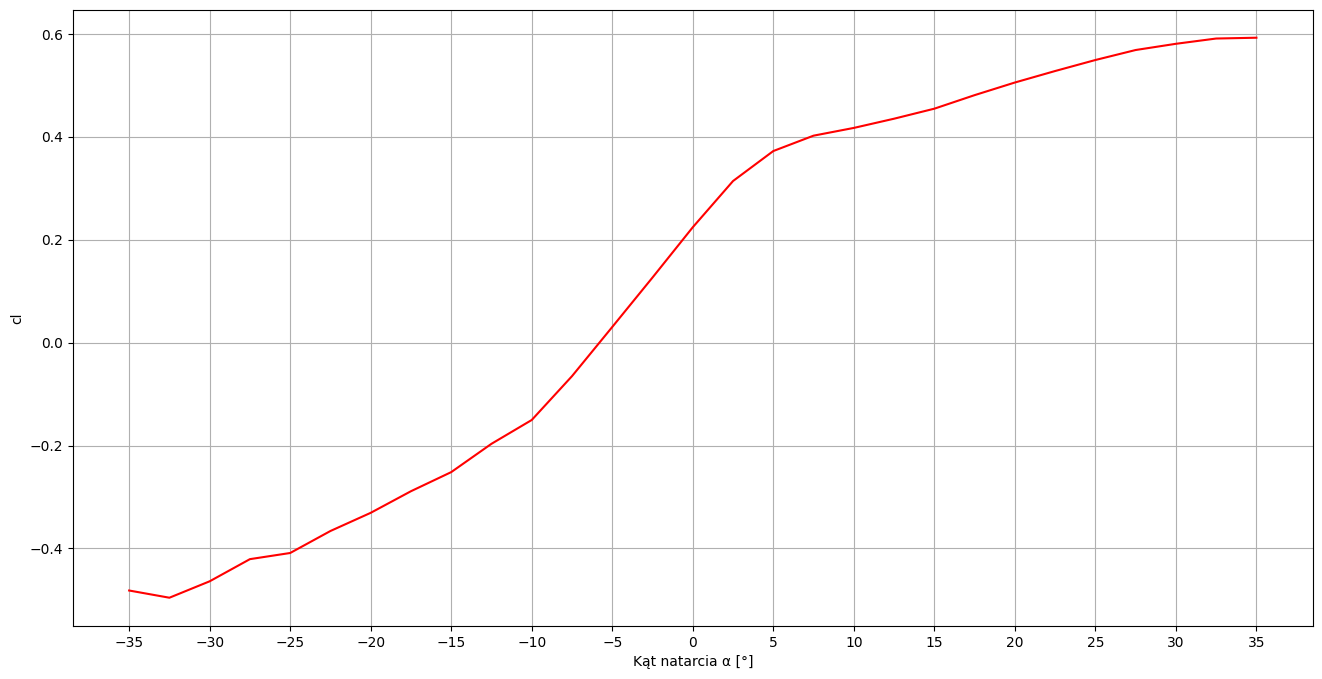
\includegraphics[width=1\linewidth]{pictures/cl-35.png}
		\caption{Wykres charakterystyki cl.}
	\end{subfigure}
	\begin{subfigure}[b]{0.4\textwidth}
		\centering
		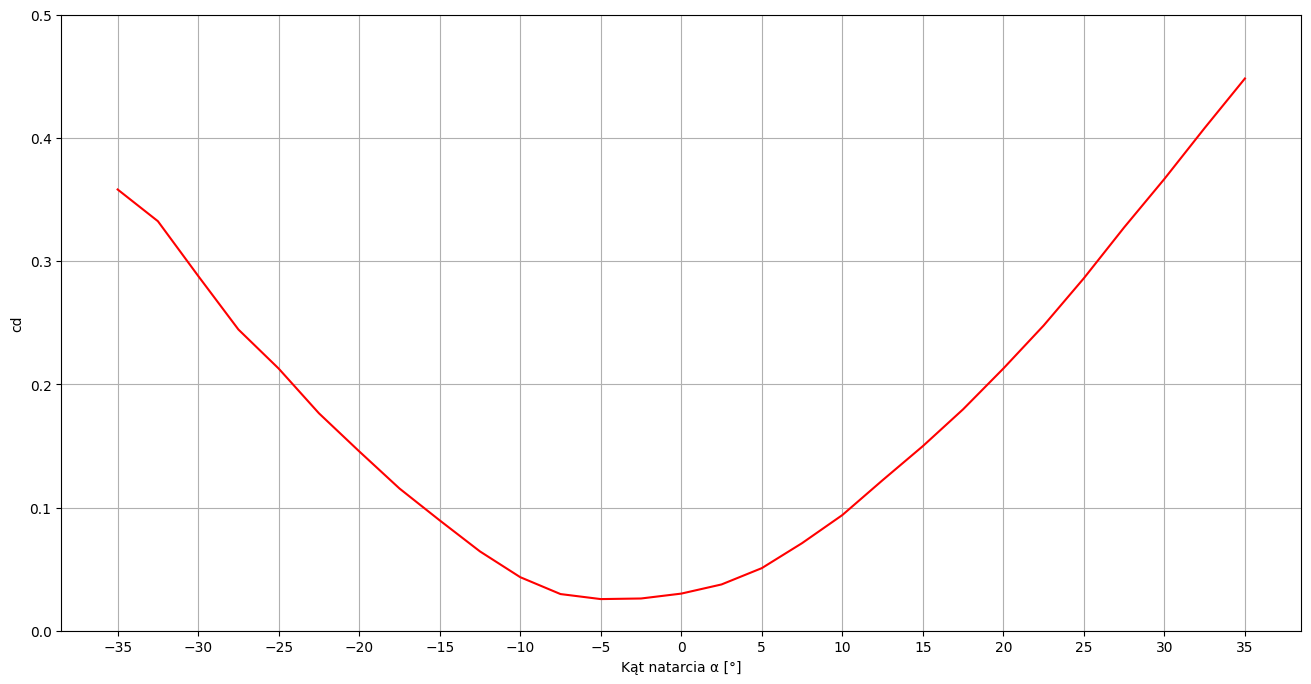
\includegraphics[width=1\linewidth]{pictures/cd-35.png}
		\caption{Wykres charakterystyki cd.}
	\end{subfigure}
	\begin{subfigure}[b]{0.4\textwidth}
		\centering
		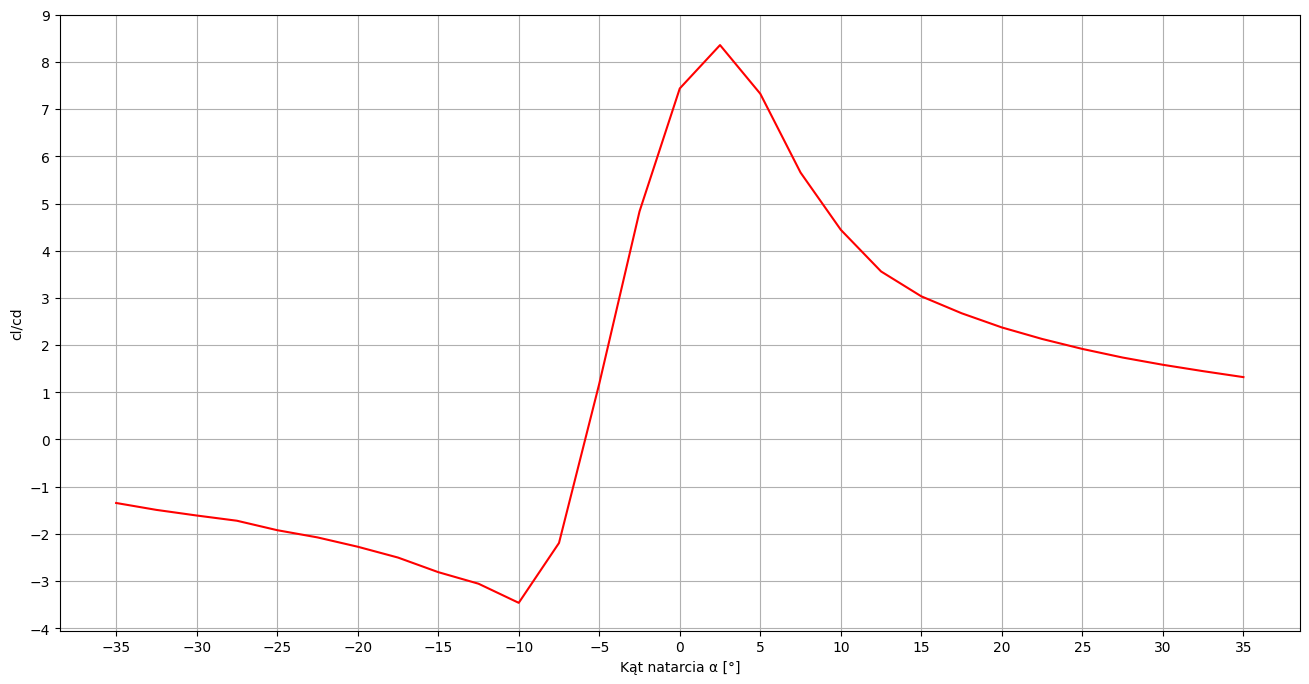
\includegraphics[width=1\linewidth]{pictures/clcd-35.png}
		\caption{Wykres charakterystyki cl/cd.}
	\end{subfigure}
	\caption{Wykresy uzyskanych charakterystyk cl, cd, cl/cd dla zakresów kąta natarcia $\alpha\in(-35^\circ, 35^\circ)$.}
	\label{fig:efficiency-graphs}
\end{figure}     

\begin{figure}[H]
	\centering
	\begin{subfigure}[b]{0.4\textwidth}
		\centering
		
\includegraphics[width=1\linewidth]{pictures/dummy.png}
		\caption{Kontury prędkości strug dla kąta $\alpha=30^\circ$}
	\end{subfigure}
	\begin{subfigure}[b]{0.4\textwidth}
		\centering
		
\includegraphics[width=1\linewidth]{pictures/dummy.png}
		\caption{Kontury rozkładu ciśnienia statycznego dla kąta $\alpha=30^\circ$}
	\end{subfigure}
	\begin{subfigure}[b]{0.4\textwidth}
		\centering
		
\includegraphics[width=1\linewidth]{pictures/dummy.png}
		\caption{Kontury rozkładu ciśnienia dynamicznego dla kąta $\alpha=30^\circ$}
	\end{subfigure}
	
	\begin{subfigure}[b]{0.4\textwidth}
		\centering
		
\includegraphics[width=1\linewidth]{pictures/dummy.png}
		\caption{Kontury prędkości strug dla kąta $\alpha=30^\circ$}
	\end{subfigure}
	\begin{subfigure}[b]{0.4\textwidth}
		\centering
		
\includegraphics[width=1\linewidth]{pictures/dummy.png}
		\caption{Kontury rozkładu ciśnienia statycznego dla kąta $\alpha=30^\circ$}
	\end{subfigure}
	\begin{subfigure}[b]{0.4\textwidth}
		\centering
		
\includegraphics[width=1\linewidth]{pictures/dummy.png}
		\caption{Kontury rozkładu ciśnienia dynamicznego dla kąta $\alpha=30^\circ$}
	\end{subfigure}
	
	\begin{subfigure}[b]{0.4\textwidth}
		\centering
		
\includegraphics[width=1\linewidth]{pictures/dummy.png}
		\caption{Kontury prędkości strug dla kąta $\alpha=30^\circ$}
	\end{subfigure}
	\begin{subfigure}[b]{0.4\textwidth}
		\centering
		
\includegraphics[width=1\linewidth]{pictures/dummy.png}
		\caption{Kontury rozkładu ciśnienia statycznego dla kąta $\alpha=30^\circ$}
	\end{subfigure}
	\begin{subfigure}[b]{0.4\textwidth}
		\centering
		
\includegraphics[width=1\linewidth]{pictures/dummy.png}
		\caption{Kontury rozkładu ciśnienia dynamicznego dla kąta $\alpha=30^\circ$}
	\end{subfigure}
	
	\begin{subfigure}[b]{0.4\textwidth}
		\centering
		
\includegraphics[width=1\linewidth]{pictures/dummy.png}
		\caption{Kontury prędkości strug dla kąta $\alpha=30^\circ$}
	\end{subfigure}
	\begin{subfigure}[b]{0.4\textwidth}
		\centering
		
\includegraphics[width=1\linewidth]{pictures/dummy.png}
		\caption{Kontury rozkładu ciśnienia statycznego dla kąta $\alpha=30^\circ$}
	\end{subfigure}
	\begin{subfigure}[b]{0.4\textwidth}
		\centering
		
\includegraphics[width=1\linewidth]{pictures/dummy.png}
		\caption{Kontury rozkładu ciśnienia dynamicznego dla kąta $\alpha=30^\circ$}
	\end{subfigure}
	
	\begin{subfigure}[b]{0.4\textwidth}
		\centering
		
\includegraphics[width=1\linewidth]{pictures/dummy.png}
		\caption{Kontury prędkości strug dla kąta $\alpha=30^\circ$}
	\end{subfigure}
	\begin{subfigure}[b]{0.4\textwidth}
		\centering
		
\includegraphics[width=1\linewidth]{pictures/dummy.png}
		\caption{Kontury rozkładu ciśnienia statycznego dla kąta $\alpha=30^\circ$}
	\end{subfigure}
	\begin{subfigure}[b]{0.4\textwidth}
		\centering
		
\includegraphics[width=1\linewidth]{pictures/dummy.png}
		\caption{Kontury rozkładu ciśnienia dynamicznego dla kąta $\alpha=30^\circ$}
	\end{subfigure}
	
	\begin{subfigure}[b]{0.4\textwidth}
		\centering
		
\includegraphics[width=1\linewidth]{pictures/dummy.png}
		\caption{Kontury prędkości strug dla kąta $\alpha=30^\circ$}
	\end{subfigure}
	\begin{subfigure}[b]{0.4\textwidth}
		\centering
		
\includegraphics[width=1\linewidth]{pictures/dummy.png}
		\caption{Kontury rozkładu ciśnienia statycznego dla kąta $\alpha=30^\circ$}
	\end{subfigure}
	\begin{subfigure}[b]{0.4\textwidth}
		\centering
		
\includegraphics[width=1\linewidth]{pictures/dummy.png}
		\caption{Kontury rozkładu ciśnienia dynamicznego dla kąta $\alpha=30^\circ$}
	\end{subfigure}
	
	\begin{subfigure}[b]{0.4\textwidth}
		\centering
		
\includegraphics[width=1\linewidth]{pictures/dummy.png}
		\caption{Kontury prędkości strug dla kąta $\alpha=30^\circ$}
	\end{subfigure}
	\begin{subfigure}[b]{0.4\textwidth}
		\centering
		
\includegraphics[width=1\linewidth]{pictures/dummy.png}
		\caption{Kontury rozkładu ciśnienia statycznego dla kąta $\alpha=30^\circ$}
	\end{subfigure}
	\begin{subfigure}[b]{0.4\textwidth}
		\centering
		
\includegraphics[width=1\linewidth]{pictures/dummy.png}
		\caption{Kontury rozkładu ciśnienia dynamicznego dla kąta $\alpha=30^\circ$}
	\end{subfigure}
	
	\caption{Wykresy uzyskanych charakterystyk cl, cd, cl/cd dla zakresów kąta natarcia $\alpha\in(-35^\circ, 35^\circ)$.}
	\label{fig:efficiency-pics}
\end{figure}    

Jak można zaobserwować na wykresach maksymalne wartości cl/cd, czyli sprawności są osiągane przy wartościach $\text{cl/cd}(\alpha=-10^\circ)=-3.5$ oraz $\text{cl/cd}(\alpha=2.5^\circ)=8.2$, przy czym do
$\alpha=\pm30^\circ$ wartości stosunku $\text{cl/cd}>1.5$. Typowe wartości cl/cd dla tego typu dronów wynoszą 1.5-5.0\cite{ugor}\cite{8014443}\cite{Graver2005UNDERWATERGD}. W związku z tym określono wartości kąta natarcia $\alpha=\pm30^\circ$ jako zakres operacyjny drona, co pokrywa się z typowymi wartościami kątów operacyjnych tego typu dronów podwodnych\cite{Jenkins2003UnderwaterGS}. Ponieważ cl/cd jest niezależne od prędkości przepływu\cite{Graver2005UNDERWATERGD} wszystkie dalsze obliczenia zostały przeprowadzone w określonym zakresie kątów natarcia.

\subsection{Symulacja w stanie ustalonym}
Ruch postępowy drona (tj - w fazie zanurzania lub wynurzania) można uogólnić jako przepływ w stanie ustalonym, tak więc w celu dalszej analizy ruchu w zależności od prędkości $\text{v}$ i kąta natarcia $\alpha$ drona przeprowadzono serię symulacji w stanie ustalonym.

W celu uzyskania dość dużego zbioru danych przeprowadzono serię symulacji dla prędkości z zakresu $\text{v}\in(0.5 \ \text{m/s}; 1.5 \ \text{m/s})$ ze skokiem między kolejnymi prędkościami $\Delta\text{v}=0.1 \ \text{m/s}$ oraz kątów natarcia w poprzednio określonym zakresie operacyjnym, czyli $\alpha\in(-30^\circ, 30^\circ)$ ze skokiem między dyskretnymi wartościami kąta równym $\Delta\alpha=2.5^\circ$. Obliczono siłę nośną $F_L$, siłę oporu $F_D$, moment pochylający $M_P$ oraz kolejno ich współczynniki: cl, cd, cm. Wyznaczono także charakterystykę stosunku cl/cd. Zbiorcze wykresy uzyskanych charakterystyk współczynników cl, cd, cm przedstawiono na rys xxx, zbiorcze wykresy sił $L$, $D$ i momentów $M$ przedstawiono na rys yyy. Poszczególne charakterystyki zestawiono w załączniku ZZZ.

\begin{figure}[H]
	\centering
	\begin{subfigure}[b]{0.4\textwidth}
		\centering
		
\includegraphics[width=1\linewidth]{pictures/dummy.png}
		\caption{Zbiorcze wykresy charakterystyk cl.}
	\end{subfigure}
	\begin{subfigure}[b]{0.4\textwidth}
		\centering
		
\includegraphics[width=1\linewidth]{pictures/dummy.png}
		\caption{Zbiorcze wykresy charakterystyk cd.}
	\end{subfigure}
	\begin{subfigure}[b]{0.4\textwidth}
		\centering
		
\includegraphics[width=1\linewidth]{pictures/dummy.png}
		\caption{Zbiorcze wykresy charakterystyk cm.}
	\end{subfigure}
	
	\caption{Zbiorcze wykresy uzyskanych charakterystyk cl, cd, cm dla wartości kąta natarcia $\alpha=(-30^\circ, 30^\circ)$.}
	\label{fig:combined-coef-graphs}
\end{figure}    

\begin{figure}[H]
	\centering
	\begin{subfigure}[b]{0.4\textwidth}
		\centering
		
\includegraphics[width=1\linewidth]{pictures/dummy.png}
		\caption{Zbiorcze wykresy charakterystyk L.}
	\end{subfigure}
	\begin{subfigure}[b]{0.4\textwidth}
		\centering
		
\includegraphics[width=1\linewidth]{pictures/dummy.png}
		\caption{Zbiorcze wykresy charakterystyk D.}
	\end{subfigure}
	\begin{subfigure}[b]{0.4\textwidth}
		\centering
		
\includegraphics[width=1\linewidth]{pictures/dummy.png}
		\caption{Zbiorcze wykresy charakterystyk M.}
	\end{subfigure}
	
	\caption{Zbiorcze wykresy uzyskanych charakterystyk L, D, M dla wartości kąta natarcia $\alpha=(-30^\circ, 30^\circ)$.}
	\label{fig:combined-force-graphs}
\end{figure}    



\subsection{Symulacja manewrów}

\subsubsection{Wariant A}
\subsubsection{Wariant B}

\subsection{Results}